\documentclass[../main.tex]{subfiles}

\begin{document}

\problem{29}
\begin{enumerate}[a)]
	\item Construct a phrase-structure grammar that generates all signed decimal numbers,
		consisting of a sign, either $+$ or $-$;
		a nonnegative integer;
		and a decimal fraction that is either the empty string or a decimal point followed by a positive integer,
		where initial zeros in an integer are allowed.
	\item Give the Backus-Naur form of this grammar.
	\item Construct a derivation tree for $-31.4$ in this grammar.
\end{enumerate}

\solution
\begin{enumerate}[a)]
	\item 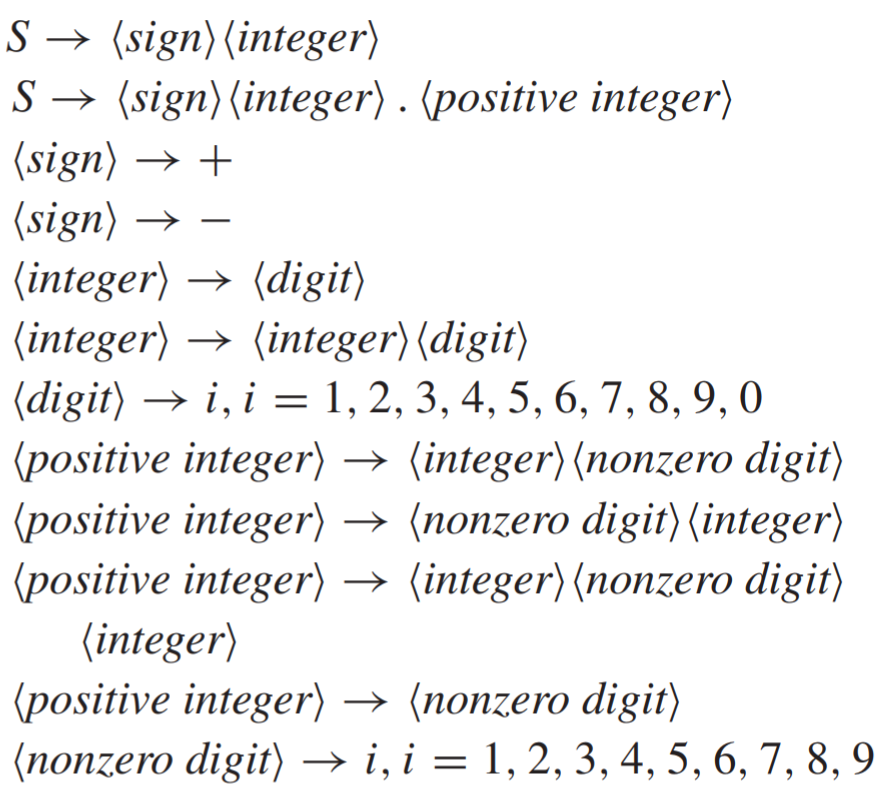
\includegraphics[scale=0.2]{img/29aA.png}
	\item 
		\begin{grammar}
			<signed decimal number> ::= <sign><integer>
			\alt <sign><integer>.<positive integer>

			<sign> ::= +|-

			<integer> ::= <digit>|<integer><digit>

			<digit> ::= 0|1|2|3|4|5|6|7|8|9

			<nonzero digit> ::= 1|2|3|4|5|6|7|8|9

			<positive integer> ::= <integer><nonzero digit>
			\alt <nonzero digit><integer>
			\alt <integer><nonzero integer><integer>
			\alt <nonzero digit>
		\end{grammar}
	\item 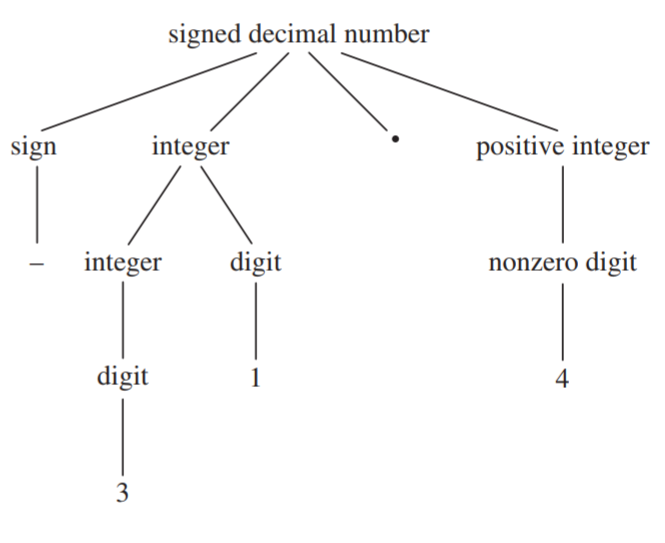
\includegraphics[scale=0.4]{img/29cA.png}
\end{enumerate}

\end{document}
